\documentclass[12pt,letterpaper]{article}

% Import packages
\usepackage{times}
\usepackage{graphicx}
\usepackage{amsmath}
\usepackage{amssymb}
\usepackage{parskip}
\usepackage{booktabs}
\usepackage[ruled,vlined]{algorithm2e}

\title{Parameterizing Curves}
\author{Alex Wong} % Put your names inside author
\date{} % Leave blank

\begin{document}

\maketitle

\section{Preliminaries}
\subsection{Vectors}

A vector is a quantity described by its magnitude and direction and can be written in the following form using its scalar components:

% About equations:
% begin and end closures lets you define equations and
% adding a label lets you refer to this equation later using \ref{label-name}
% slashes give you new lines and
% ampersand lets you add another element on the same line
\begin{equation}
\label{eqn:vector-example}
    \overrightarrow{v} = \begin{bmatrix} 3 \\ 4 \\ 5 \end{bmatrix} \\
    \text{ , } \\
    \overrightarrow{u} = \begin{bmatrix} 3 & 4 & 5 \end{bmatrix}
\end{equation}

% Dollar sign closures lets you enter math mode (equivalent to equations above)
% Notice that the rendered PDF has a slightly different font
$\overrightarrow{v}$ is a $3 \times 1$ vector or equivalently a $3 \times 1$ matrix, comprised of three rows and one column. $\overrightarrow{u}$ is similarly a $1 \times 3$ vector or matrix (one row and three columns). Aside from the form they are written in, $\overrightarrow{v}$ and $\overrightarrow{u}$ are equivalent.
Vectors are closed under addition:

\begin{equation}
    \overrightarrow{v} = \overrightarrow{v_{1}} + \overrightarrow{v_{2}} 
\end{equation}

and scalar multiplication for some constant $c$:

\begin{equation}
    \overrightarrow{v} = c\overrightarrow{v_{1}} 
\end{equation}

which means that both the sum of two vectors and a vector multiplied by a scalar will result in a new vector.

\subsection{Unit Vectors}

Unit vectors are vectors with lengths or magnitudes of $1$. To convert a vector into a unit vector, we simply normalize the vector by its length or magnitude:

\begin{equation}
    \hat{\overrightarrow{v}} = \frac{\overrightarrow{v}}{||\overrightarrow{v}||} \text{ for } ||\overrightarrow{v}|| \\
    \text{ is length or magnitude (norm) of } \overrightarrow{v}
\end{equation}

\subsection{Vector Transpose}

The transpose of a vector is trivially flipping its rows and columns and denoted with the superscript $\intercal$:

\begin{equation}
    \overrightarrow{v} = \begin{bmatrix} 3 \\ 4 \\ 5 \end{bmatrix} \\
    \text{ , } \\
    \overrightarrow{v}^{\intercal} = \begin{bmatrix} 3 & 4 & 5 \end{bmatrix} \\
    \text{ , } \\
    (\overrightarrow{v}^{\intercal})^{\intercal} = \begin{bmatrix} 3 \\ 4 \\ 5 \end{bmatrix}
\end{equation}

The transpose of a transposed vector $\overrightarrow{v}$ gives the original $\overrightarrow{v}$. $\overrightarrow{u}$ from Eqn. \ref{eqn:vector-example} is in fact $\overrightarrow{v}^{\intercal}$. 
Note that the transpose of a matrix is slightly more complicated, but is no more than flipping a matrix across its diagonal.

\subsection{Dot Product (Inner Product)}

The dot product of two vectors $\overrightarrow{v}$ and $ \overrightarrow{u}$ is the summation over the component-wise multiplication of the two vectors:

\begin{equation}
    \overrightarrow{v} \cdot \overrightarrow{u} = \\
    v_{0} \cdot u_{0} + \\
    v_{1} \cdot u_{1} + \\
    ... 
    v_{N} \cdot u_{N} \\
    \text{ for } N \text{ elements }
\end{equation}

which can be equivalently written as:

\begin{equation}
    \overrightarrow{v} \cdot \overrightarrow{u} = \sum^{N}_{i=0} v_{i}u_{i}
\end{equation}

Hence, the dot product of two vectors results in a scalar. 

Let $\overrightarrow{v}$ and $\overrightarrow{u}$ be:

\begin{equation}
    \overrightarrow{v} = \begin{bmatrix} 1 & 2 & 3 \end{bmatrix} \\
    \text{ , } \\
    \overrightarrow{u} = \begin{bmatrix} 4 \\ 5 \\ 6 \end{bmatrix}
\end{equation}

Then the dot product of $\overrightarrow{v}$ and $\overrightarrow{u}$ is:

\begin{equation}
\overrightarrow{v} \cdot \overrightarrow{u} = \begin{bmatrix} 1 & 2 & 3 \end{bmatrix} \cdot \begin{bmatrix} 4 \\ 5 \\ 6 \end{bmatrix} = 1 \cdot 4 + 2 \cdot 5 + 3 \cdot 6 = 32
\end{equation}

Note that the dot product of two vector written in this form (each element in  gives some insight on matrix multiplication as they are now both performing row element multiplied by column element).

\section{Parameterizing a Line}

Suppose we have a point $p_{0}$ and a vector $\overrightarrow{v}$, we can form a new point $p_{1}$ by simply adding $p_{0}$ with $\overrightarrow{v}$:

\begin{equation}
    p_{1} = p_{0} + \overrightarrow{v}
\end{equation}

Consequently, we can subtract $p_{1}$ by $p_{0}$ to form the vector $\overrightarrow{v}$:

\begin{equation}
    \overrightarrow{v} = p_{1} - p_{0}
\end{equation}

% figure closures let you import figures into your file
% [h] means to try to place the figure here (or latex will choose where it best fits)
% [!] means disregard what latex thinks looks best
% Create a folder on the left panel called figures and place your figures inside
% You may reference them using the path figures/figure_name
% center or centering closures centers your figure to the horizontally
% Captions goes below the text
% You can also add a label to the figure
\begin{figure*}[!h]
    \begin{center}
        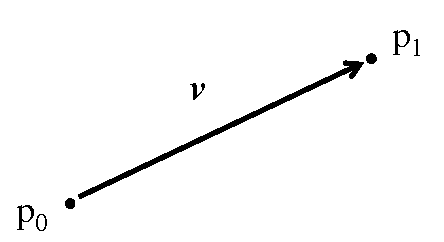
\includegraphics[width=0.33\textwidth]{figures/01_vector}
    \end{center}
    \caption{Points $p_{0}$, $p_{1}$ and the vector $\overrightarrow{v}$.}
    \label{fig:vector-example}
\end{figure*}

Now suppose that we would like to parameterize the line formed by $p_{0}$ and $p_{1}$ using a variable $t$ such that given $p_{0}$, $p_{1}$ and $t$ we will be able to know every point $p$ along the line formed by $p_{1} - p_{0}$.

\begin{figure*}[!h]
    \begin{center}
        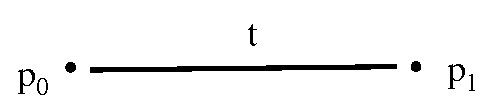
\includegraphics[width=0.33\textwidth]{figures/01_line_param_t}
    \end{center}
    \caption{Points $p_{0}$, $p_{1}$ and the parameter $t$ define a line.}
\end{figure*}

If we treat $t$ as a scale or ratio between $p_{0}$, $p_{1}$ then we can write this as

\begin{equation}
\label{eqn:line-param-t}
    p = p_{0} + t(p_{1} - p_{0}) \text{ for } t \in [0, 1]
\end{equation}

If $t = 0$ then $p = p_{0}$ and if $t = 1$ then $p = p_{1}$. We naturally get the midpoint between the $p_{0}$ and $p_{1}$ if we were to select $t = 0.5$, $p = 0.5p_{0}+0.5p_{1}$. If we were to sample (or select different values of) $t$, then we can interpolate all points along the line. Note, we must have the constraint that $t \in [0, 1]$ or the interpolated points will go outside of the line defined by $p_{0}$ and $p_{1}$.

% Abbreviate reference to equation as Eqn., figure as Fig., and table as Tab.
We will now rewrite Eqn. \ref{eqn:line-param-t} in a slightly different form such that we can then motivate using coefficients in front of our points.
\begin{equation}
    p = (1 - t)p_{0} + tp_{1} \text{ for } t \in [0, 1]
\end{equation}

We can now in fact substitute $(1 - t)$ and $t$ with $t_{0}$ and $t_{1}$ to write:

\begin{equation}
    p = t_{0}p_{0} + t_{1}p_{1} \text{ for } t_{0} + t_{1} = 1
\end{equation}

with the new constraint that the sum of the coefficients must sum up to 1. The constraint that we have set explicitly restricts any points we produce using the above equations to live within the space between the two points. 

This is known as an affine combination and the space that these points exists in (or is defined by the vectors) is known as an affine space, which in summary:

\begin{equation}
    p = p_{0} + t\overrightarrow{v} = p_{0} + t(p_{1} - p_{0}) = (1 - t)p_{0} + tp_{1} = t_{0}p_{0} + t_{1}p_{1}
\end{equation}

for $t \in [0, 1]$ and $t_{0} + t_{1} = 1$.

\section{Parameterizing a Curve}

Thus far, we know that a by parameterizing a line using two points and a parameter that scales between the two points given some constraint, we are able to obtain every point on the line. Since a line can be parameterized by two points, we can extend the concept to a parameterize a plane using three points:

\begin{figure*}[!h]
    \begin{center}
        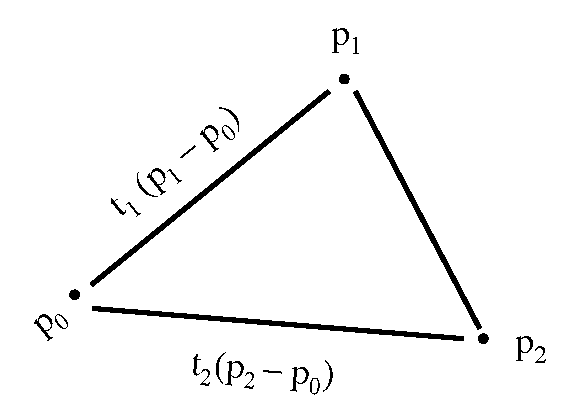
\includegraphics[width=0.40\textwidth]{figures/01_triangle_param_t}
    \end{center}
    \caption{Points $p_{0}$, $p_{1}, p_{2}$ define a plane (a triangle) }
\end{figure*}

This allows us to write the following to describe any point within the triangle:

\begin{equation}
    p = p_{0} + t_{1}(p_{1} - p_{0}) + t_{2}(p_{2} - p_{0})
\end{equation}

and equivalently:

\begin{equation}
    p = (1 - t_{1} - t_{2})p_{0} + t_{1}p_{1} + t_{2}p_{2}
\end{equation}

We  then substitute $t_0 = (1 - t_{1} - t_{2})$ to arrive at the same form we have written for our equation of a line with the constraint that $t_{0}$, $t_{1}$, $t_{2}$ must sum to 1:

\begin{equation}
    p = t_{0}p_{0} + t_{1}p_{1} + t_{2}p_{2} \text{ for } t_{0} + t_{1} + t_{2} = 1
\end{equation}

We can view each $t_{0}$, $t_{1}$, $t_{2}$ as the coordinates of the plane (in this case it is a triangle) contained within $p_{0}$, $p_{1}$, $p_{2}$. By varying the coordinates we can obtain a new point on the plane. These coordinates are known Barycentric coordinates, which are specific to a triangle -- meaning we can parameterize any triangle using the above form. We can utilize this knowledge to form a curved line.

Thus far, we have seen first order polynomials (which we know are linear and hence a line) as coefficients (coordinates) to the space defined by the give points. To form curves (e.g. a parabola), we know that we will need at least second order polynomials (quadratics). Let's consider the following polynomials:

% The aligned closure lets you align multiple equations based on the position
% of the ampersand sign
% In this case they are all aligned at the equal symbol
\begin{equation}
    \begin{aligned}
    	(1 - t)^{2} &= 1 - 2t + t^{2} \\
    	2t(1-t) &= 0 + 2t - 2t^{2} \\
    	t^{2} &= 0 + 0 + t^{2}
    \end{aligned}
\end{equation}

Based on their expansions, we see that $(1 - 2t + t^2) + (2t - 2t^2) + t^2 = 1$, which suggests that we can use these polynomials in forming our affine combination for three points (a plane), which allows for curvature. 

\begin{equation}
    p = (1 - t)^{2}p_{0} + 2t(1-t)p_{1} + t^{2}p_{2} \text{ for } t \in [0, 1]
\end{equation}

We substitute $t_{0} = (1 - t)^{2}$, $t_{1} = 2t(1-t)$, $t_{2} = t^{2}$ with the constraint that $t \in [0, 1]$. We can see that if $t = 0$ then $p = p_{0}$ and if $t = 1$ then $p = p_{2}$ -- guaranteeing that our point will live within the triangle. The second order terms further tell us that we will have a curve (barring co-linear points).

\begin{figure*}[!h]
    \begin{center}
        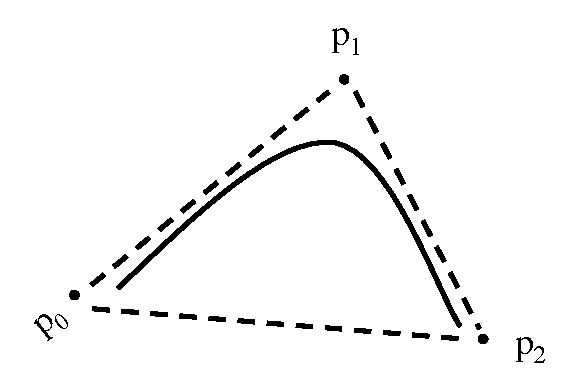
\includegraphics[width=0.40\textwidth]{figures/01_curve_3}
    \end{center}
    \caption{Illustration of the curve formed by $p = (1 - t)^{2}p_{0} + 2t(1-t)p_{1} + t^{2}p_{2}$. Dashed lines mark the bounds of the triangle defined by $p_{0}$, $p_{1}$, and $p_{2}$.}
\end{figure*}

Note that such a curve is bounded within $p_{0}$, $p_{1}$, and $p_{2}$ meaning that $t$ must satisfy the constraint $t \in [0, 1]$. Not all polynomials satisfy this constraint. A polynomial satisfying this constraint is known as a Bernstein Polynomial. Such polynomials exist in higher orders as well, allowing us to draw curves with multiple inflection points (which generally correspond to the one less than the order).

Now let's suppose we have the following Bernstein polynomial:

\begin{equation}
    \begin{aligned}
    	(1 - t)^{3} &= 1 - 3t + 3t^{2} - t^{3} \\
    	3t(1-t)^{2} &= 0 + 3t - 6t^{2} + 3t^{3} \\
    	3t^{2}(1-t) &= 0 + 0 + 3t^{2} - 3t^{3} \\
    	t^{3} &= 0 + 0 + 0 + t^{3}
    \end{aligned}
\end{equation}

This again sums to one and satisfies our constraint; hence, we can use these polynomials as our coefficients for an equation with four points $p_{0}$, $p_{1}$, $p_{2}$, and $p_{3}$:

\begin{equation}
\label{eqn:bernstein-4}
    p = (1 - t)^{3}p_{0} + 3t(1-t)^{2}p_{1} + 3t^{2}(1-t)p_{2} + t^{3}p_{3} \text{ for } t \in [0, 1]
\end{equation}

We again observe that if $t = 0$ then $p = p_{0}$ and if $t = 1$ then $p = p_{3}$. As the expansion of these polynomials can become quite messy, we will now modify our notation by writing the expansion into vector form. 

\begin{equation}
    p = \begin{bmatrix} 1 - 3t + 3t^{2} - t^{3} & 3t - 6t^{2} + 3t^{3} & 3t^{2} - 3t^{3} & t^{3} \end{bmatrix} \\
    \cdot \\
    \begin{bmatrix} p_{0} \\ p_{1} \\ p_{2} \\ p_{3} \end{bmatrix}
\end{equation}

We can see that the dot product of the two vectors would give us the expanded version of Eqn. \ref{eqn:bernstein-4}. Let's further decompose the coefficients by separating each scalar from the parameter $t$, where each column corresponds one polynomial (e.g. column one contains the coefficients of $(1 - t)^{3} = 1 - 3t + 3t^{2} - t^{3}$:

\begin{equation}
    p = \begin{bmatrix} 1 & t & t^{2} & t^{3} \end{bmatrix} \\
    \begin{bmatrix} 1 & 0 & 0 & 0 \\ -3 & 3 & 0 & 0 \\ 3 & -6 & 3  & 0 \\ -1 & 3 & -3 & 1 \end{bmatrix} \\
    \cdot \\
    \begin{bmatrix} p_{0} \\ p_{1} \\ p_{2} \\ p_{3} \end{bmatrix}
\end{equation}

We have just written our vector space as a matrix. The first (left-most) $1 \times 4$ vector (matrix) contains the orders of $t$, which gives us a sense of the number of inflection points in the curve. The center $4 \times 4$ matrix is known as a transformation matrix as it will tell us how points on the curve will deform (i.e. stretch in certain directions). The final $4 \times 1$ matrix gives us the space that the curve exists. 

\end{document}
